\documentclass[sigconf]{acmart}
\AtBeginDocument{%
  \providecommand\BibTeX{{%
    \normalfont B\kern-0.5em{\scshape i\kern-0.25em b}\kern-0.8em\TeX}}}
\setcopyright{rightsretained}
\acmConference[SNACS '22]{Social Network Analysis for Computer Scientists Course 2022}{Master CS, Fall 2022}{Leiden, the Netherlands}
\copyrightyear{2022}
\acmYear{2022}
\acmISBN{}
\acmDOI{}
\usepackage[braket, qm]{qcircuit}
%%%% Do not modify lines 1-11

\begin{document}

\title{Your Original and Relevant Course Project Title}
\subtitle{ Social Network Analysis for Computer Scientists --- Course paper} % do not modify thi

\author{Student name 1}
%\orcid{0000-0001-5468-1030}
\email{student2@umail.leidenuniv.nl}
\affiliation{
  \institution{LIACS, Leiden University}
  \city{Leiden}
  \country{Netherlands}}

\author{Student name 2}
%\orcid{0000-0001-5468-1030}
\email{student2@umail.leidenuniv.nl}
\affiliation{
  \institution{LIACS, Leiden University}
  \city{Leiden}  
  \country{Netherlands}}

\renewcommand{\shortauthors}{Lastname1 and Lastname2}

\keywords{keyword1, keyword2, keyword3, social network analysis, network science}

\begin{abstract}

% the abstract summarizes the entire paper: context, problem, solution, approach, data, experimental results, conclusion and real-world implications. but, shortly, so in half a column or so.

\end{abstract}

\maketitle

\section{Introduction}

% textual description of the context, the problem considered, why it is important, how it is addressed in other works, and what real-world applications are. end with a paragraph on what the contributions of the paper are (so, which problems you solve or which research questions you address), and finally a paragraph on how the remainder of the paper is organized.

\section{Related work}

% briefly discuss other papers related to this work, or previous work describing other approaches for the same problem. end with a statement on how your paper contributes to these works.



\section{Approach}

\subsection{Variational Quantum Classifier}
Variational Quantum Classifier(VQC) is a kind of parameterized quantum circuit used in classification tasks \cite{havlivcek2019supervised}. Conventional machine learning methods, such as SVM and neural networks, often take advantage of a parameterized model as classifiers. During training process, these methods use a target function or loss function to measure the difference between prediction results and ground true labels and update the parameters in the model to improve its performance. After several training epochs on adequate data, these machine learning methods can achieve great performance on prediction on unseen data as well. VQC works in a similar way, whereas applying a quantum circuit as its parameterized model. The abstract model of VQC is shown in Figure \ref{fig:VQC}, including data encoding (or feature mapping) $U_{enc}(x)$, variational model $U_{train}(\theta)$, measurement, and parameter updating(usually via gradient decent). In the following subsection 3.1.1 to 3.1.4, we will introduce these processing steps in detail. And then, in subsection 3.1.5, the overall working principle of our VQC circuit will be discussed.
\begin{figure}[!ht]
	\centering
	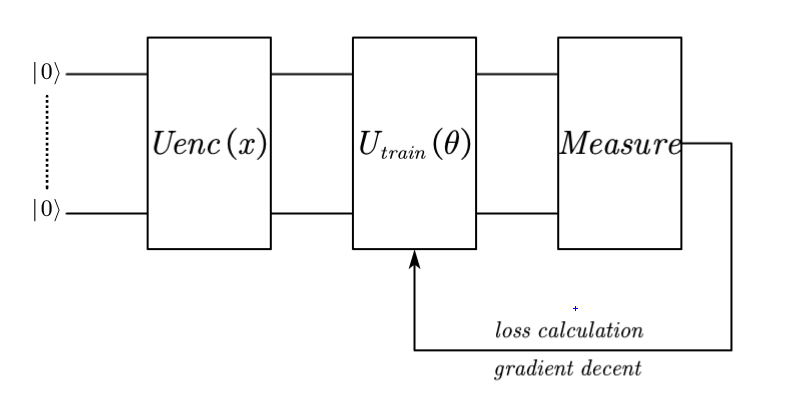
\includegraphics[width=0.48\textwidth]{VQC.png}
	\caption{Abstract model of VQC: {\small \textnormal{ A Variational Quantum Classifier contains these processing steps: data encoding, varational model, measurement and parameter updating.}} }
	\label{fig:VQC}
\end{figure}

\subsubsection{Data Encoding}\hfill\\
As what we have discussed above, VQC attempts to apply parameterized quantum circuit as its learning model. However, nowadays most of data is stored in classical computers which quantum circuit cannot directly access to. Hence, it's necessary to encode classical data into quantum state that can be preocessed by quantum circuit at first. 

There are many basic methods to achieve this encoding preocess, such as basis encoding, amplitude encoding and angle encoding. Besides, several higher order encoding methods which combines different basic encoding methods are studied as well. In this paper, our proposal data encoding method is xxxx, one of the most popular higher order encoding methods. The specific quantum circuit $U_{enc}(x)$ is shown in Figure \ref{fig:encoding} (2-qubit case). As we can see, in this 2-qubit example, the encoding circuit is simplely composed of two Hamdamard gates, three phase gates with the components of the input data $x$ as their parameter and two $CNOT$ gates as the entangling gate. Due to difference of the input data components of each class, the states produced by this circuit will be different as well. In addition, because of the use of entangling gate, the $CNOT$, the state on each qubit will have interaction. Besides, the initial quantum state of each qubit is $\ket{0}$ on account of the requirement of real quantum computers.
\begin{figure}[!ht]
	\centering
	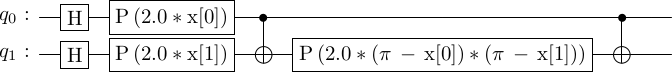
\includegraphics[width=0.48\textwidth]{encode.png}
	\caption{Data encoding circuit: {\small \textnormal{Specific quantum circuit of data encoding in 2-qubit case. This circuit is composed of Hamdamard gates, phase gates, and entangling gate($CNOT$).}} }
	\label{fig:encoding}
\end{figure}
\subsubsection{Variational Model}\hfill\\
Variational model is a quantum circuit with trainalbe parameters. During the training process, these parameters will be updated to improve the model's performance. There are various kinds of variational model can be applied in VQC. In this paper, the circuit of our variational model $U_{train}(\theta)$is shown in Figure \ref{fig:variational} (2-qubit case). This 2-qubit example is composed by four y-axis rotation gates parameterized by $\theta$ which is the parameter set to be trained, and one controlled Z gate as the entangling gate. After training, these parameterized rotation gates along with entangling gate can have the ability to convert input states of diverse classes to different output states which can be measured to make a final prediction.   
\begin{figure}[!ht]
	\centering
	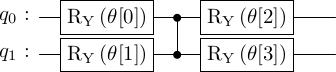
\includegraphics[width=0.48\textwidth]{vari.png}
	\caption{Variational model circuit: {\small \textnormal{Specific quantum circuit of variational model in 2-qubit case. This circuit is composed of parameterized y-axis rotation gates and controlled Z gate.}} }
	\label{fig:variational}
\end{figure}
\subsubsection{Measurement}\hfill\\
 When training most of machine learning models, we need to compare the prediction results and the labels to update parameters, which works the same way in VQC. Nevertheless, after data encoding and variational model, the results are still in quantum states. Hence, we need to extract prediction results from these quantum states. This process is accomplished by measurement. We simply measure all qubits in the circuit and run the circuit for many times. Then we can obtain a distribution of these possible results.
 
 In binary classification tasks, a common way to extract prediction results is to converge the result states distribution into a binary distribution of odd parity states and even parity states. In other words, we consider the parity distribution as the prediction probability of two classes. For example, we run a 2-qubit circuit for 100 times and obtain the measurement result which is [00:21, 01:33, 10:28, 11:18], so the prediction probability for each class shall be [0.39, 0.61]. Therefore, the second class will be predicted as the final result.
\subsubsection{Parameter Updating}\hfill\\
Parameter updating process is the most significant part of machine learning, which includes loss calculation and gradient decent. Loss calculation is the same as the conventional machine learning. When we obtain the predcition probability distribution of each class, we compare the difference between it and ground true label through a loss function. Despite popularity of cross entropy loss in classification tasks, we still choose MAE loss in our model.

In the conventional machine learning, such as neural network, gradient decent based method is famous and efficient to update parameters in the training process. However, it's hard to calculate gradient as in the conventional machine learning due to the fact that our model is based on the quantum circuit. Hence, \cite{schuld2020circuit} proposed a method using difference to subsitute real gradients. In detail, for each parameter $\theta$, we run the circuit and calculate the loss value based on the prediction probability distribution results for parameter $\theta+s$ and $\theta-s$, namely $L(\theta+s)$ and $L(\theta-s)$. Then using the following formula to calculate the gradient:
$$gradient(\theta)=\frac{L(\theta+s)-L(\theta-s)}{2s}$$ 
where $s$ is usually chosen as a small real positive number. Then this proximate gradient is used to update model's parameters just as the same way in the conventional machine learning.

\subsubsection{Overall Analysis}\hfill\\
In this subsection, we make a overal analysis on our VQC and the circuit theoretically to illustrate why this process makes a good classifier.

According to the analysis in the previous subsections, our  ansatz can be written in the mathematical form:
$$U(x,\theta)=U_{train}(\theta)U_{enc}(x)$$

Before the measurement, the following state is prepared:
$$\ket{\psi(x,\theta)}=U(x,\theta)\ket{0^n}$$

And then we measure the observable $Z^{\otimes n}$ on the above state to implement the function:
$$f_\theta(x)=\bra{\psi(x,\theta)}Z^{\otimes n}\ket{\psi(x,\theta)}$$  

This function is actually the expectation of the observing result distribution on the computational basis of even parity states and odd parity states, when giving even parity states value 1 (represent class 0) and odd parity states value -1 (represent class 1). To be more specific, let us use a 2-qubit example to illustrate it.

Suppose we have a general 2-qubit state $\ket{\phi}=a\ket{00}+b\ket{01}+c\ket{10}+d\ket{11}$ as $\ket{\psi(x,\theta)}$. Feed this state into the above function, and the result is actually computed as:
\begin{align*}
	f_\theta(x)&=\bra{\phi}Z^{\otimes n}\ket{\phi}\\
	&=\begin{pmatrix}
		a & b & c & d
		\end{pmatrix}\begin{pmatrix}
		1 & 0 & 0 & 0 \\
		0 & -1 & 0 & 0 \\
		0 & 0 & -1 & 0 \\
		0 & 0 & 0 & 1 
	\end{pmatrix}\begin{pmatrix}
	a \\
	b \\
	c \\
	d 
	\end{pmatrix}\\
    &=a^2-b^2-c^2+d^2
\end{align*}
When we observe $\ket{\phi}$ on the computational basis, the final probability to obtain odd and even parity state shall be:
$$p(even)=p(\ket{00})+p(\ket{11})=a^2+d^2$$
$$p(odd)=p(\ket{01})+p(\ket{10})=b^2+c^2$$

Remember we have given even parity states value 1 and odd parity states value -1 to make it a classifier, so the expectation value of this probability distribution will be:
$$E=1*p(even)+(-1)*p(odd)=a^2-b^2-c^2+d^2$$

It's actually the same result compared to $f_{\theta}(x)$. However, in real cases, we couldn't calculate the exact expectation while adequate repeatation of running the circuit can give us the precise enough approxiamate result. In other words, when we repeat the circuit for enough times, the obtained result distribution can be considered as the real distribution.

Finally, we turn the function $f_{\theta}(x)$ into a (binary) classifier by considering its sign:
$$
h_{\theta}(x)=sign(f_{\theta}(x))=\left\{
\begin{aligned}
	1  & \quad if \ f_{\theta}(x)>0 \\
	-1  & \quad if \ f_{\theta}(x)<0 
\end{aligned}
\right.
$$

Therefore, through adjusting the value of parameter $\theta$ via training process, the input data of different classes will finally have different $h_{\theta}(x)$ function values which makes it an effective classifier.

Finally, our VQC circuit (in 2-qubit case) is shown in Figure \ref{fig:whole}. It combines the  processing steps which have been discussed above. In section 5, we will show and discuss the experimental results of this VQC circuit on different datasets.
\begin{figure*}[!ht]
	\centering
	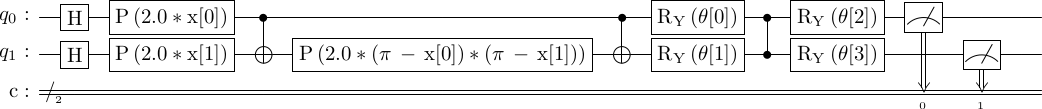
\includegraphics[width=0.9\textwidth]{whole.png}
	\caption{VQC quantum circuit: {\small \textnormal{Our final variational quantum classifier circuit in 2-qubit case. Notice that the initial quantum state of each qubit is always $\ket{0}$.}} }
	\label{fig:whole}
\end{figure*}

\subsection{Quantum Circuit Partitioning}
Quantum circuit partitioning is technique to evaluate a large quantum circuit only using smaller quantum computer with fewer quantum qubits \cite{marshall2022high}. Many quantum algorithms require more qubits than nowaday quantum computer can really provide, which is a tremendous limitation for designing quantum algorithm. The quantum circuit partition method provides a practical solution to this problem. It divides a larger quantum circuit into several smaller parts which can be run and evaluate individually. Then these results are combined in a polynomial to replicate the output of the larger machine. Various methods of circuit partitioning have been developed to simulate large quantum circuit with fewer qubits, though these methods require more evaluation running times on these divided smaller circuits. In this paper, we mainly apply two methods which are proposed in paper \cite{marshall2022high} and \cite{mitarai2021constructing}.

\subsubsection{}\hfill\\
The first method in paper \cite{marshall2022high} divides the larger circuit into smaller blocks, and for each block of partition, a new parameterized unitary is added with different parameters $\xi$.

\section{Data}



% what datasets did you use, what types of networks do they represent, where did you obtain the data? did you do any processing? give a table describing data characteristics, such as number of nodes, edges, average degree, etc.

\section{Experiments}

% subsections on for example the experimental setup (which software, hardware and parameters did you choose), as well as the results of applying your approach to the data you described in preceding sections, leading to results that answer your research questions. you likely present some tables and figures

\section{Conclusion}

% summarize in at most one column the main results of the paper, stating how you addressed the problem statement and how the experiments help understand whether  the approach works (or not). end with one or two short suggestions for future work. 

\begin{acks}
% optional: acknowledgments, so people or organizations you wish to thank 
\end{acks}


\bibliographystyle{ACM-Reference-Format}
\bibliography{snacspaper} % put your references in bibtex format in snacspaper.bib

%\appendix
%\section{Robustness checks}
% Appendixes are optional for the course project. they can contain proofs, figures or tables that do not fit in the main body of the text, but are handy as background information

\end{document}
\endinput
